% Options for packages loaded elsewhere
\PassOptionsToPackage{unicode}{hyperref}
\PassOptionsToPackage{hyphens}{url}
%
\documentclass[
  11pt,
]{article}
\usepackage{lmodern}
\usepackage{amssymb,amsmath}
\usepackage{ifxetex,ifluatex}
\ifnum 0\ifxetex 1\fi\ifluatex 1\fi=0 % if pdftex
  \usepackage[T1]{fontenc}
  \usepackage[utf8]{inputenc}
  \usepackage{textcomp} % provide euro and other symbols
\else % if luatex or xetex
  \usepackage{unicode-math}
  \defaultfontfeatures{Scale=MatchLowercase}
  \defaultfontfeatures[\rmfamily]{Ligatures=TeX,Scale=1}
\fi
% Use upquote if available, for straight quotes in verbatim environments
\IfFileExists{upquote.sty}{\usepackage{upquote}}{}
\IfFileExists{microtype.sty}{% use microtype if available
  \usepackage[]{microtype}
  \UseMicrotypeSet[protrusion]{basicmath} % disable protrusion for tt fonts
}{}
\makeatletter
\@ifundefined{KOMAClassName}{% if non-KOMA class
  \IfFileExists{parskip.sty}{%
    \usepackage{parskip}
  }{% else
    \setlength{\parindent}{0pt}
    \setlength{\parskip}{6pt plus 2pt minus 1pt}}
}{% if KOMA class
  \KOMAoptions{parskip=half}}
\makeatother
\usepackage{xcolor}
\IfFileExists{xurl.sty}{\usepackage{xurl}}{} % add URL line breaks if available
\IfFileExists{bookmark.sty}{\usepackage{bookmark}}{\usepackage{hyperref}}
\hypersetup{
  pdftitle={Series Temporales - Trabajo Final},
  pdfauthor={Esteban Schab - Anabella De Battista},
  hidelinks,
  pdfcreator={LaTeX via pandoc}}
\urlstyle{same} % disable monospaced font for URLs
\usepackage[margin=1in]{geometry}
\usepackage{color}
\usepackage{fancyvrb}
\newcommand{\VerbBar}{|}
\newcommand{\VERB}{\Verb[commandchars=\\\{\}]}
\DefineVerbatimEnvironment{Highlighting}{Verbatim}{commandchars=\\\{\}}
% Add ',fontsize=\small' for more characters per line
\usepackage{framed}
\definecolor{shadecolor}{RGB}{248,248,248}
\newenvironment{Shaded}{\begin{snugshade}}{\end{snugshade}}
\newcommand{\AlertTok}[1]{\textcolor[rgb]{0.94,0.16,0.16}{#1}}
\newcommand{\AnnotationTok}[1]{\textcolor[rgb]{0.56,0.35,0.01}{\textbf{\textit{#1}}}}
\newcommand{\AttributeTok}[1]{\textcolor[rgb]{0.77,0.63,0.00}{#1}}
\newcommand{\BaseNTok}[1]{\textcolor[rgb]{0.00,0.00,0.81}{#1}}
\newcommand{\BuiltInTok}[1]{#1}
\newcommand{\CharTok}[1]{\textcolor[rgb]{0.31,0.60,0.02}{#1}}
\newcommand{\CommentTok}[1]{\textcolor[rgb]{0.56,0.35,0.01}{\textit{#1}}}
\newcommand{\CommentVarTok}[1]{\textcolor[rgb]{0.56,0.35,0.01}{\textbf{\textit{#1}}}}
\newcommand{\ConstantTok}[1]{\textcolor[rgb]{0.00,0.00,0.00}{#1}}
\newcommand{\ControlFlowTok}[1]{\textcolor[rgb]{0.13,0.29,0.53}{\textbf{#1}}}
\newcommand{\DataTypeTok}[1]{\textcolor[rgb]{0.13,0.29,0.53}{#1}}
\newcommand{\DecValTok}[1]{\textcolor[rgb]{0.00,0.00,0.81}{#1}}
\newcommand{\DocumentationTok}[1]{\textcolor[rgb]{0.56,0.35,0.01}{\textbf{\textit{#1}}}}
\newcommand{\ErrorTok}[1]{\textcolor[rgb]{0.64,0.00,0.00}{\textbf{#1}}}
\newcommand{\ExtensionTok}[1]{#1}
\newcommand{\FloatTok}[1]{\textcolor[rgb]{0.00,0.00,0.81}{#1}}
\newcommand{\FunctionTok}[1]{\textcolor[rgb]{0.00,0.00,0.00}{#1}}
\newcommand{\ImportTok}[1]{#1}
\newcommand{\InformationTok}[1]{\textcolor[rgb]{0.56,0.35,0.01}{\textbf{\textit{#1}}}}
\newcommand{\KeywordTok}[1]{\textcolor[rgb]{0.13,0.29,0.53}{\textbf{#1}}}
\newcommand{\NormalTok}[1]{#1}
\newcommand{\OperatorTok}[1]{\textcolor[rgb]{0.81,0.36,0.00}{\textbf{#1}}}
\newcommand{\OtherTok}[1]{\textcolor[rgb]{0.56,0.35,0.01}{#1}}
\newcommand{\PreprocessorTok}[1]{\textcolor[rgb]{0.56,0.35,0.01}{\textit{#1}}}
\newcommand{\RegionMarkerTok}[1]{#1}
\newcommand{\SpecialCharTok}[1]{\textcolor[rgb]{0.00,0.00,0.00}{#1}}
\newcommand{\SpecialStringTok}[1]{\textcolor[rgb]{0.31,0.60,0.02}{#1}}
\newcommand{\StringTok}[1]{\textcolor[rgb]{0.31,0.60,0.02}{#1}}
\newcommand{\VariableTok}[1]{\textcolor[rgb]{0.00,0.00,0.00}{#1}}
\newcommand{\VerbatimStringTok}[1]{\textcolor[rgb]{0.31,0.60,0.02}{#1}}
\newcommand{\WarningTok}[1]{\textcolor[rgb]{0.56,0.35,0.01}{\textbf{\textit{#1}}}}
\usepackage{graphicx,grffile}
\makeatletter
\def\maxwidth{\ifdim\Gin@nat@width>\linewidth\linewidth\else\Gin@nat@width\fi}
\def\maxheight{\ifdim\Gin@nat@height>\textheight\textheight\else\Gin@nat@height\fi}
\makeatother
% Scale images if necessary, so that they will not overflow the page
% margins by default, and it is still possible to overwrite the defaults
% using explicit options in \includegraphics[width, height, ...]{}
\setkeys{Gin}{width=\maxwidth,height=\maxheight,keepaspectratio}
% Set default figure placement to htbp
\makeatletter
\def\fps@figure{htbp}
\makeatother
\setlength{\emergencystretch}{3em} % prevent overfull lines
\providecommand{\tightlist}{%
  \setlength{\itemsep}{0pt}\setlength{\parskip}{0pt}}
\setcounter{secnumdepth}{-\maxdimen} % remove section numbering

\title{Series Temporales - Trabajo Final}
\author{Esteban Schab - Anabella De Battista}
\date{Febrero 2021}

\begin{document}
\maketitle

{
\setcounter{tocdepth}{2}
\tableofcontents
}
\clearpage

\hypertarget{ejercicio-1---modelos-arma}{%
\section{Ejercicio 1 - Modelos ARMA}\label{ejercicio-1---modelos-arma}}

Se requiere:

\begin{enumerate}
\def\labelenumi{\alph{enumi}.}
\item
  Identificación del modelo empleando los primeros 140 registros
  mediante ACF, PACF y AIC.
\item
  Realizar un pronóstico out-of sample, sobre los últimos 10 datos.
  Determinar la precisión del pronóstico de los dos mejores modelos
  calculados en en apartado (a), mediante el error cuadrático medio
  (mean squared error) y el error absoluto medio (mean absolute error).
\end{enumerate}

\hypertarget{modelo-2}{%
\section{Modelo 2}\label{modelo-2}}

\begin{Shaded}
\begin{Highlighting}[]
\NormalTok{modelo2 <-}\StringTok{ }\KeywordTok{read.csv}\NormalTok{(}\StringTok{"./data/modelo2.csv"}\NormalTok{, }\DataTypeTok{header =} \OtherTok{TRUE}\NormalTok{, }\DataTypeTok{sep =} \StringTok{","}\NormalTok{, }\DataTypeTok{quote =} \StringTok{"}\CharTok{\textbackslash{}"}\StringTok{"}\NormalTok{, }
                    \DataTypeTok{dec =} \StringTok{"."}\NormalTok{, }\DataTypeTok{fill =} \OtherTok{TRUE}\NormalTok{)}
\NormalTok{m2_ts <-}\StringTok{ }\KeywordTok{ts}\NormalTok{(modelo2[,}\DecValTok{2}\NormalTok{])}
\end{Highlighting}
\end{Shaded}

\hypertarget{estaduxedsticas-principales}{%
\subsection{Estadísticas
principales}\label{estaduxedsticas-principales}}

\begin{Shaded}
\begin{Highlighting}[]
\KeywordTok{summary}\NormalTok{(m2_ts)}
\end{Highlighting}
\end{Shaded}

\begin{verbatim}
##     Min.  1st Qu.   Median     Mean  3rd Qu.     Max. 
## -3.17920 -0.94755 -0.09789 -0.21507  0.53178  2.32752
\end{verbatim}

\hypertarget{gruxe1fico-de-la-serie-temporal}{%
\subsection{Gráfico de la serie
temporal}\label{gruxe1fico-de-la-serie-temporal}}

\begin{center}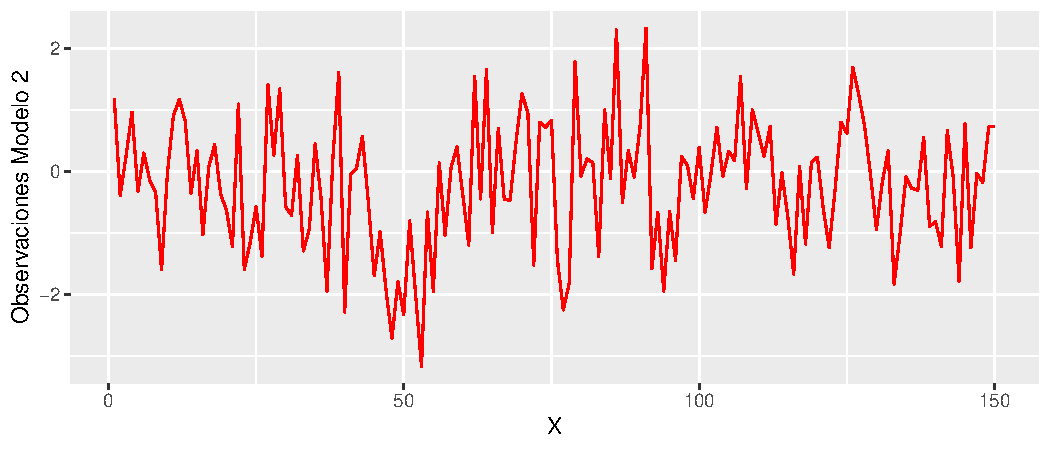
\includegraphics[width=0.9\linewidth]{RmdFigs/plot_ts2-1} \end{center}

En base al gráfico la serie aparenta ser constante en media y en
varianza, por lo que se podría pensar que es estacionaria.

\hypertarget{histograma}{%
\subsubsection{Histograma}\label{histograma}}

\begin{Shaded}
\begin{Highlighting}[]
\KeywordTok{hist}\NormalTok{(m2_ts, }\DataTypeTok{prob=}\OtherTok{TRUE}\NormalTok{, }\DataTypeTok{main =} \StringTok{"Histograma Modelo 2"}\NormalTok{, }\DataTypeTok{xlab =} \StringTok{"x"}\NormalTok{, }\DataTypeTok{ylab =} \StringTok{"frecuencia"}\NormalTok{)}
\NormalTok{x <-}\StringTok{ }\KeywordTok{seq}\NormalTok{(}\KeywordTok{min}\NormalTok{(m2_ts), }\KeywordTok{max}\NormalTok{(m2_ts), }\DataTypeTok{length =} \DecValTok{40}\NormalTok{)}
\NormalTok{f <-}\StringTok{ }\KeywordTok{dnorm}\NormalTok{(x, }\DataTypeTok{mean =} \KeywordTok{mean}\NormalTok{(m2_ts), }\DataTypeTok{sd =} \KeywordTok{sd}\NormalTok{(m2_ts))}
\KeywordTok{lines}\NormalTok{(x, f, }\DataTypeTok{col =} \StringTok{"red"}\NormalTok{, }\DataTypeTok{lwd =} \DecValTok{2}\NormalTok{)}
\end{Highlighting}
\end{Shaded}

\begin{center}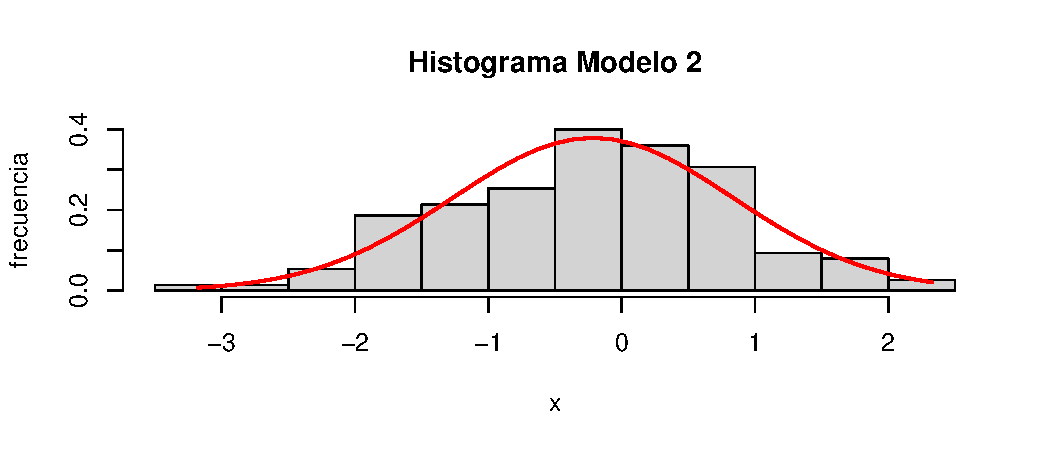
\includegraphics[width=0.9\linewidth]{RmdFigs/histograma_m2-1} \end{center}

En base al histograma se ve que la distribución de los datos se ajusta a
una curva normal.

\hypertarget{gruxe1ficas-acf-y-pacf}{%
\subsubsection{Gráficas ACF y PACF}\label{gruxe1ficas-acf-y-pacf}}

\begin{Shaded}
\begin{Highlighting}[]
\KeywordTok{acf}\NormalTok{(m2_ts, }\DataTypeTok{main =} \StringTok{"ACF - Modelo 2"}\NormalTok{)}
\end{Highlighting}
\end{Shaded}

\begin{center}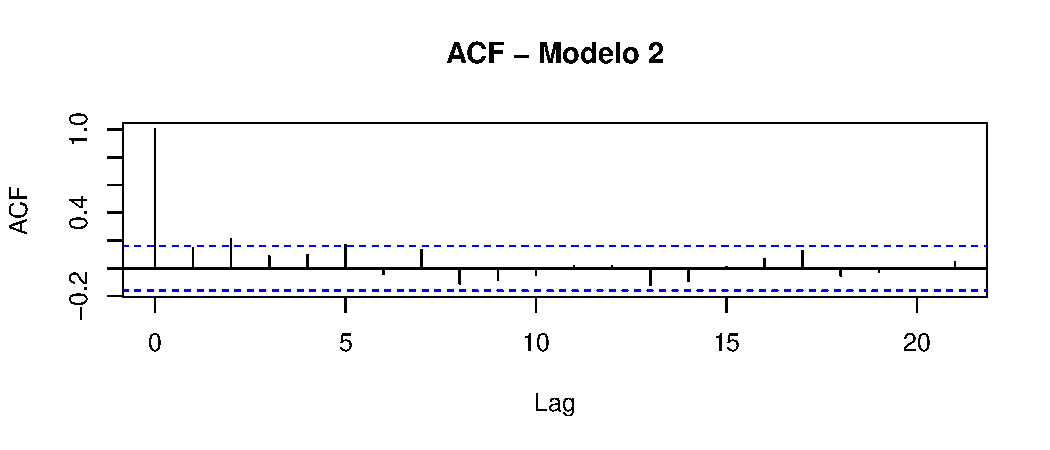
\includegraphics[width=0.9\linewidth]{RmdFigs/acfM2-1} \end{center}

\begin{Shaded}
\begin{Highlighting}[]
\KeywordTok{pacf}\NormalTok{(m2_ts, }\DataTypeTok{main =} \StringTok{"PACF - Modelo 2"}\NormalTok{)}
\end{Highlighting}
\end{Shaded}

\begin{center}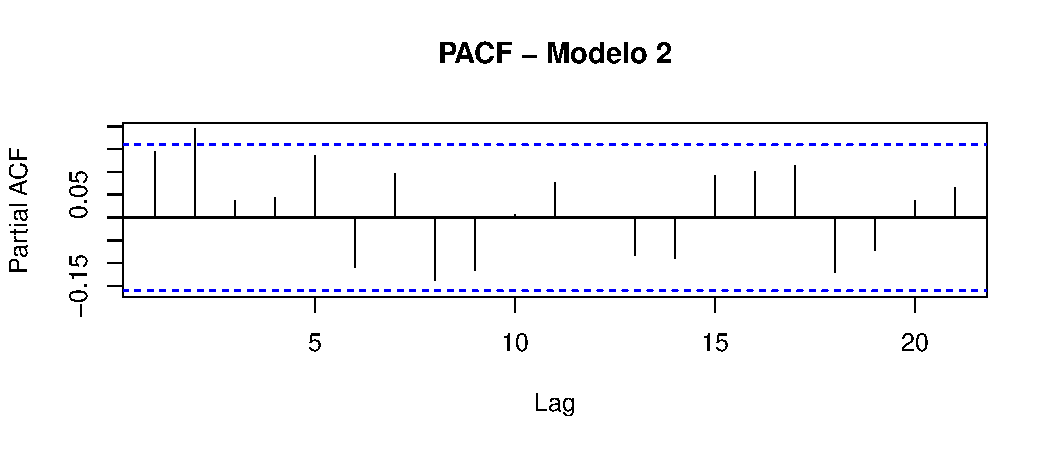
\includegraphics[width=0.9\linewidth]{RmdFigs/pacfM2-1} \end{center}

De acuerdo al gráfico de autocorrelación se puede apreciar que la serie
es estacionaria ya que la función decae a medida que aumentan los
rezagos en el tiempo. No existe componente estacional.

Si se analizan las gráficas ACF y PACF se deduce que es posible plantear
varios modelos tentativos para el análisis, realizando combinaciones de
p y q entre 0 y 2.

Previamente se descarta que exista componente estacional en la serie de
datos.

\begin{Shaded}
\begin{Highlighting}[]
\NormalTok{fit <-}\StringTok{ }\KeywordTok{tbats}\NormalTok{(m2_ts)}
\NormalTok{s <-}\StringTok{ }\OperatorTok{!}\KeywordTok{is.null}\NormalTok{(fit}\OperatorTok{$}\NormalTok{seasonal)}
\NormalTok{s}
\end{Highlighting}
\end{Shaded}

\begin{verbatim}
## [1] FALSE
\end{verbatim}

El hecho de que \textbf{s=FALSE} indica que no hay estacionalidad en la
serie de tiempo modelo2.

\hypertarget{verificaciuxf3n-de-que-la-serie-es-estacionaria}{%
\subsection{Verificación de que la serie es
estacionaria}\label{verificaciuxf3n-de-que-la-serie-es-estacionaria}}

Aplicamos el test de estacionariedad ADF (Dickey-Fuller).

Planteamiento de Hipótesis Significancia \(\alpha\) = 0.05 H0: La serie
es no estacionaria: tiene raíz unitaria H1: La serie es estacionaria: no
tiene raíz unitaria

\begin{Shaded}
\begin{Highlighting}[]
\KeywordTok{library}\NormalTok{(tseries)}
\NormalTok{adf<-}\KeywordTok{adf.test}\NormalTok{(m2_ts)}
\NormalTok{adf}\OperatorTok{$}\NormalTok{p.value}
\end{Highlighting}
\end{Shaded}

\begin{verbatim}
## [1] 0.01
\end{verbatim}

Se aplica el test KPSS para verificar si la serie es estacionaria.

\begin{Shaded}
\begin{Highlighting}[]
\NormalTok{kpss<-}\KeywordTok{kpss.test}\NormalTok{(m2_ts)}
\NormalTok{kpss}\OperatorTok{$}\NormalTok{p.value}
\end{Highlighting}
\end{Shaded}

\begin{verbatim}
## [1] 0.1
\end{verbatim}

Como el p-valor del Test de Dickey-Fuller da menor que \(\alpha\) y en
el caso del test KPSS da mayor que \(\alpha\), concluimos que la serie
\emph{es estacionaria}.

\hypertarget{configuraciuxf3n-de-paruxe1metros-para-procesos-arma-variando-p-y-q.}{%
\subsection{Configuración de parámetros para procesos ARMA, variando p y
q.}\label{configuraciuxf3n-de-paruxe1metros-para-procesos-arma-variando-p-y-q.}}

\begin{Shaded}
\begin{Highlighting}[]
\NormalTok{p.maximo <-}\StringTok{ }\DecValTok{2}  \CommentTok{# orden maximo p }
\NormalTok{q.maximo <-}\StringTok{ }\DecValTok{2}  \CommentTok{# orden maximo q }
\NormalTok{cantidad.modelos <-}\StringTok{ }\NormalTok{(p.maximo}\OperatorTok{+}\DecValTok{1}\NormalTok{)}\OperatorTok{*}\NormalTok{(q.maximo}\OperatorTok{+}\DecValTok{1}\NormalTok{)  }

\CommentTok{#combinaciones de p y q}
\NormalTok{orden.modelos <-}\StringTok{ }\KeywordTok{permutations}\NormalTok{(p.maximo}\OperatorTok{+}\DecValTok{1}\NormalTok{,}\DecValTok{2}\NormalTok{,}\DecValTok{0}\OperatorTok{:}\NormalTok{p.maximo,}\DataTypeTok{repeats.allowed =} \OtherTok{TRUE}\NormalTok{) }
\NormalTok{resumen<-}\StringTok{ }\KeywordTok{matrix}\NormalTok{(}\DecValTok{0}\NormalTok{,cantidad.modelos,}\DecValTok{6}\NormalTok{)  }\CommentTok{#matriz resumen (loglik, sigma2 y aic)}
\KeywordTok{colnames}\NormalTok{(resumen) <-}\StringTok{ }\KeywordTok{c}\NormalTok{(}\StringTok{"Loglik"}\NormalTok{,}\StringTok{"Sigma2"}\NormalTok{,}\StringTok{"AIC"}\NormalTok{,}\StringTok{"AIC diff"}\NormalTok{,}
                       \StringTok{"Likelihood_model"}\NormalTok{,}\StringTok{"Akaike weights"}\NormalTok{)}
 \CommentTok{#nombre de las filas}
\NormalTok{nombres <-}\StringTok{ }\KeywordTok{matrix}\NormalTok{(}\DecValTok{0}\NormalTok{,}\DecValTok{1}\NormalTok{,cantidad.modelos)}
\ControlFlowTok{for}\NormalTok{ (modelo.numero }\ControlFlowTok{in} \DecValTok{1}\OperatorTok{:}\NormalTok{cantidad.modelos)\{}
\NormalTok{  nombres[}\DecValTok{1}\NormalTok{,modelo.numero] <-}\StringTok{ }\KeywordTok{paste}\NormalTok{(}\StringTok{"p="}\NormalTok{,}\KeywordTok{as.character}\NormalTok{(orden.modelos[modelo.numero,}\DecValTok{1}\NormalTok{]),}
                                    \StringTok{"q="}\NormalTok{,}\KeywordTok{as.character}\NormalTok{(orden.modelos[modelo.numero,}\DecValTok{2}\NormalTok{]))}
\NormalTok{\}}
\KeywordTok{rownames}\NormalTok{(resumen) <-}\StringTok{ }\NormalTok{nombres}
\end{Highlighting}
\end{Shaded}

\hypertarget{prueba-de-los-modelos-con-los-primeros-140-valores-de-la-serie.}{%
\subsection{Prueba de los modelos con los primeros 140 valores de la
serie.}\label{prueba-de-los-modelos-con-los-primeros-140-valores-de-la-serie.}}

\begin{Shaded}
\begin{Highlighting}[]
\NormalTok{fit_m2_ts <-}\StringTok{ }\KeywordTok{window}\NormalTok{(m2_ts, }\DataTypeTok{start=}\DecValTok{1}\NormalTok{, }\DataTypeTok{end=}\DecValTok{140}\NormalTok{)}

\NormalTok{residuos.modelos <-}\StringTok{ }\KeywordTok{matrix}\NormalTok{(}\DecValTok{0}\NormalTok{,}\KeywordTok{length}\NormalTok{(fit_m2_ts),cantidad.modelos)}
\KeywordTok{colnames}\NormalTok{(residuos.modelos)<-}\StringTok{ }\NormalTok{nombres}
\NormalTok{celda <-}\StringTok{ }\DecValTok{0}
\ControlFlowTok{for}\NormalTok{(p }\ControlFlowTok{in} \DecValTok{0}\OperatorTok{:}\NormalTok{p.maximo)\{}
  \ControlFlowTok{for}\NormalTok{(q }\ControlFlowTok{in} \DecValTok{0}\OperatorTok{:}\NormalTok{q.maximo)\{}
\NormalTok{    celda=}\StringTok{ }\NormalTok{celda}\OperatorTok{+}\DecValTok{1}   
\NormalTok{    AR2 <-}\StringTok{ }\KeywordTok{arima}\NormalTok{(fit_m2_ts, }\DataTypeTok{order =} \KeywordTok{c}\NormalTok{(p,}\DecValTok{0}\NormalTok{,q))}
\NormalTok{    residuos.modelos[,celda] <-}\StringTok{ }\NormalTok{AR2}\OperatorTok{$}\NormalTok{residuals}
\NormalTok{    resumen[celda,}\DecValTok{1}\NormalTok{] <-}\StringTok{ }\NormalTok{AR2}\OperatorTok{$}\NormalTok{loglik}
\NormalTok{    resumen[celda,}\DecValTok{2}\NormalTok{] <-}\StringTok{ }\NormalTok{AR2}\OperatorTok{$}\NormalTok{sigma2}
\NormalTok{    resumen[celda,}\DecValTok{3}\NormalTok{] <-}\StringTok{ }\NormalTok{AR2}\OperatorTok{$}\NormalTok{aic}
\NormalTok{  \}\}}
\NormalTok{resumen[,}\DecValTok{4}\NormalTok{]<-resumen[,}\DecValTok{3}\NormalTok{]}\OperatorTok{-}\KeywordTok{min}\NormalTok{(resumen[,}\DecValTok{3}\NormalTok{])}
\NormalTok{resumen[,}\DecValTok{5}\NormalTok{]<-}\KeywordTok{exp}\NormalTok{(}\OperatorTok{-}\FloatTok{0.5}\OperatorTok{*}\NormalTok{resumen[,}\DecValTok{4}\NormalTok{])}
\NormalTok{resumen[,}\DecValTok{6}\NormalTok{]<-resumen[,}\DecValTok{5}\NormalTok{]}\OperatorTok{/}\KeywordTok{sum}\NormalTok{(resumen[,}\DecValTok{5}\NormalTok{])}

\CommentTok{# resumen de resultados}
\KeywordTok{round}\NormalTok{(resumen,}\DataTypeTok{digits=}\DecValTok{4}\NormalTok{) }
\end{Highlighting}
\end{Shaded}

\begin{verbatim}
##              Loglik Sigma2      AIC AIC diff Likelihood_model Akaike weights
## p= 0 q= 0 -206.6337 1.1208 417.2675   5.2932           0.0709         0.0187
## p= 0 q= 1 -205.2406 1.0986 416.4813   4.5071           0.1050         0.0277
## p= 0 q= 2 -202.5139 1.0561 413.0277   1.0535           0.5905         0.1560
## p= 1 q= 0 -204.6809 1.0897 415.3618   3.3876           0.1838         0.0486
## p= 1 q= 1 -202.2367 1.0518 412.4735   0.4993           0.7791         0.2058
## p= 1 q= 2 -201.8525 1.0459 413.7051   1.7309           0.4209         0.1112
## p= 2 q= 0 -201.9871 1.0480 411.9742   0.0000           1.0000         0.2642
## p= 2 q= 1 -201.7812 1.0448 413.5625   1.5882           0.4520         0.1194
## p= 2 q= 2 -201.6831 1.0434 415.3663   3.3921           0.1834         0.0484
\end{verbatim}

En base a los resultados se aprecia que para el dasaset \emph{modelo2},
los dos mejores modelos son: arma7: ARMA(2,0) cuyo valor para \emph{AIC
diff} es = 0.0000 y arma5: ARMA(1,1) cuyo valor para \emph{AIC diff} es
= 0.4993.

Para validar el modelo se grafica el correlograma de los residuos para
comprobar que son ruido blanco.

\begin{Shaded}
\begin{Highlighting}[]
\CommentTok{# Calculo ACF y PACF para el mejor modelo ARMA para el dataset modelo2}
\NormalTok{res_m2_arma7 <-}\StringTok{ }\NormalTok{residuos.modelos[,}\DecValTok{7}\NormalTok{]}
\KeywordTok{acf2}\NormalTok{(res_m2_arma7)}
\end{Highlighting}
\end{Shaded}

\begin{center}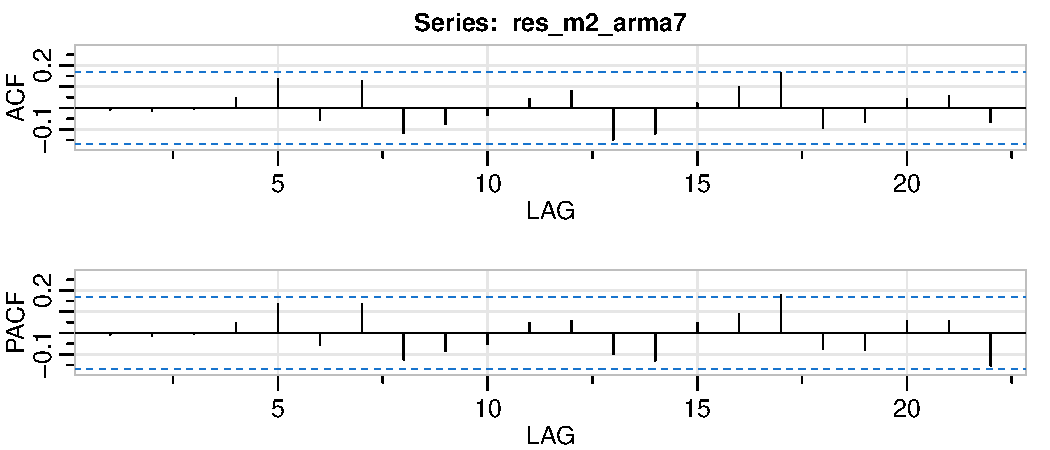
\includegraphics[width=0.9\linewidth]{RmdFigs/acf2_arma7-1} \end{center}

\begin{verbatim}
##       [,1]  [,2] [,3] [,4] [,5]  [,6] [,7]  [,8]  [,9] [,10] [,11] [,12] [,13]
## ACF  -0.01 -0.01    0 0.04 0.13 -0.06 0.13 -0.12 -0.08 -0.03  0.04  0.08 -0.15
## PACF -0.01 -0.01    0 0.04 0.13 -0.05 0.13 -0.12 -0.08 -0.05  0.04  0.05 -0.10
##      [,14] [,15] [,16] [,17] [,18] [,19] [,20] [,21] [,22]
## ACF  -0.12  0.02  0.10  0.16 -0.09 -0.07  0.04  0.05 -0.07
## PACF -0.13  0.05  0.09  0.18 -0.08 -0.08  0.06  0.05 -0.15
\end{verbatim}

En los correlogramas se aprecia que no hay ningún rezago significativo
por lo que se puede decir que los residuos son ruido blanco.

\hypertarget{prueba-con-la-funciuxf3n-auto.arima}{%
\subsection{Prueba con la función
auto.arima}\label{prueba-con-la-funciuxf3n-auto.arima}}

La función auto.arima permite determinar el mejor modelo ARIMA para un
conjunto de datos. Al ejecutarla en este caso coinicide con el modelo
identificado previamente.

\begin{Shaded}
\begin{Highlighting}[]
  \KeywordTok{auto.arima}\NormalTok{(fit_m2_ts, }\DataTypeTok{stepwise =} \OtherTok{FALSE}\NormalTok{, }\DataTypeTok{approximation =} \OtherTok{FALSE}\NormalTok{)}
\end{Highlighting}
\end{Shaded}

\begin{verbatim}
## Series: fit_m2_ts 
## ARIMA(2,0,0) with non-zero mean 
## 
## Coefficients:
##          ar1     ar2     mean
##       0.1338  0.1946  -0.2174
## s.e.  0.0830  0.0830   0.1281
## 
## sigma^2 estimated as 1.071:  log likelihood=-201.99
## AIC=411.97   AICc=412.27   BIC=423.74
\end{verbatim}

Por lo tanto estamos en condiciones de realizar un pronóstico para las
siguientes 10 observaciones de la serie.

\hypertarget{pronuxf3stico-para-modelo-2-con-arma20}{%
\subsection{Pronóstico para Modelo 2 con
ARMA(2,0)}\label{pronuxf3stico-para-modelo-2-con-arma20}}

\begin{Shaded}
\begin{Highlighting}[]
\CommentTok{#parametros p y q del mejor modelo}
\NormalTok{p <-}\StringTok{ }\DecValTok{2}
\NormalTok{q <-}\StringTok{ }\DecValTok{0}
\CommentTok{#fiteo el modelo con 140 datos (para despues hacer el out-of-sample forecast)}
\NormalTok{sample.fin <-}\StringTok{ }\DecValTok{140}
\NormalTok{AR2_}\DecValTok{20}\NormalTok{ <-}\StringTok{ }\KeywordTok{arima}\NormalTok{(m2_ts[}\DecValTok{1}\OperatorTok{:}\NormalTok{sample.fin], }\DataTypeTok{order =} \KeywordTok{c}\NormalTok{(p,}\DecValTok{0}\NormalTok{,q))}
\KeywordTok{ts.plot}\NormalTok{(m2_ts[}\DecValTok{1}\OperatorTok{:}\DecValTok{150}\NormalTok{])}
\end{Highlighting}
\end{Shaded}

\begin{center}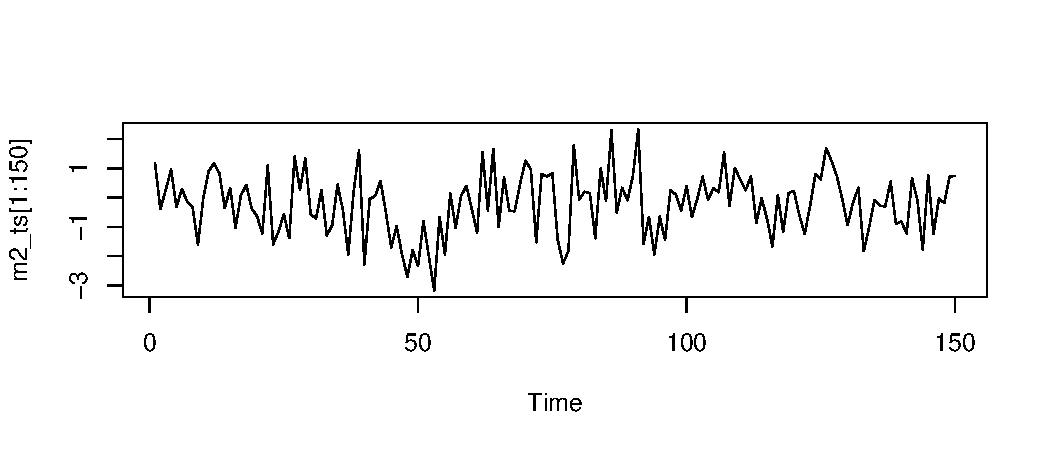
\includegraphics[width=0.9\linewidth]{RmdFigs/fit_1_m2-1} \end{center}

\begin{Shaded}
\begin{Highlighting}[]
\CommentTok{#plotting the m2_ts series plus the forecast and 95% prediction intervals}
\KeywordTok{ts.plot}\NormalTok{(m2_ts[}\DecValTok{1}\OperatorTok{:}\NormalTok{sample.fin], }\DataTypeTok{xlim =} \KeywordTok{c}\NormalTok{(}\DecValTok{1}\NormalTok{, sample.fin))}
\NormalTok{AR2_}\DecValTok{20}\NormalTok{_forecast <-}\StringTok{ }\KeywordTok{predict}\NormalTok{(AR2_}\DecValTok{20}\NormalTok{, }\DataTypeTok{n.ahead =} \KeywordTok{length}\NormalTok{(m2_ts)}\OperatorTok{-}\NormalTok{sample.fin)}\OperatorTok{$}\NormalTok{pred}
\NormalTok{AR2_}\DecValTok{20}\NormalTok{_forecast_se <-}\StringTok{ }\KeywordTok{predict}\NormalTok{(AR2_}\DecValTok{20}\NormalTok{, }\DataTypeTok{n.ahead =} \KeywordTok{length}\NormalTok{(m2_ts)}\OperatorTok{-}\NormalTok{sample.fin)}\OperatorTok{$}\NormalTok{se}
\KeywordTok{points}\NormalTok{(AR2_}\DecValTok{20}\NormalTok{_forecast, }\DataTypeTok{type =} \StringTok{"l"}\NormalTok{, }\DataTypeTok{col =} \DecValTok{3}\NormalTok{)}
\KeywordTok{points}\NormalTok{(AR2_}\DecValTok{20}\NormalTok{_forecast }\OperatorTok{-}\StringTok{ }\DecValTok{2}\OperatorTok{*}\NormalTok{AR2_}\DecValTok{20}\NormalTok{_forecast_se, }\DataTypeTok{type =} \StringTok{"l"}\NormalTok{, }\DataTypeTok{col =} \DecValTok{2}\NormalTok{, }\DataTypeTok{lty =} \DecValTok{2}\NormalTok{)}
\KeywordTok{points}\NormalTok{(AR2_}\DecValTok{20}\NormalTok{_forecast }\OperatorTok{+}\StringTok{ }\DecValTok{2}\OperatorTok{*}\NormalTok{AR2_}\DecValTok{20}\NormalTok{_forecast_se, }\DataTypeTok{type =} \StringTok{"l"}\NormalTok{, }\DataTypeTok{col =} \DecValTok{2}\NormalTok{, }\DataTypeTok{lty =} \DecValTok{2}\NormalTok{)}
\KeywordTok{points}\NormalTok{(sample.fin}\OperatorTok{+}\DecValTok{1}\OperatorTok{:}\DecValTok{150}\NormalTok{,m2_ts[sample.fin}\OperatorTok{+}\DecValTok{1}\OperatorTok{:}\DecValTok{150}\NormalTok{], }\DataTypeTok{type =} \StringTok{"l"}\NormalTok{, }\DataTypeTok{col =} \DecValTok{2}\NormalTok{)}
\end{Highlighting}
\end{Shaded}

\begin{center}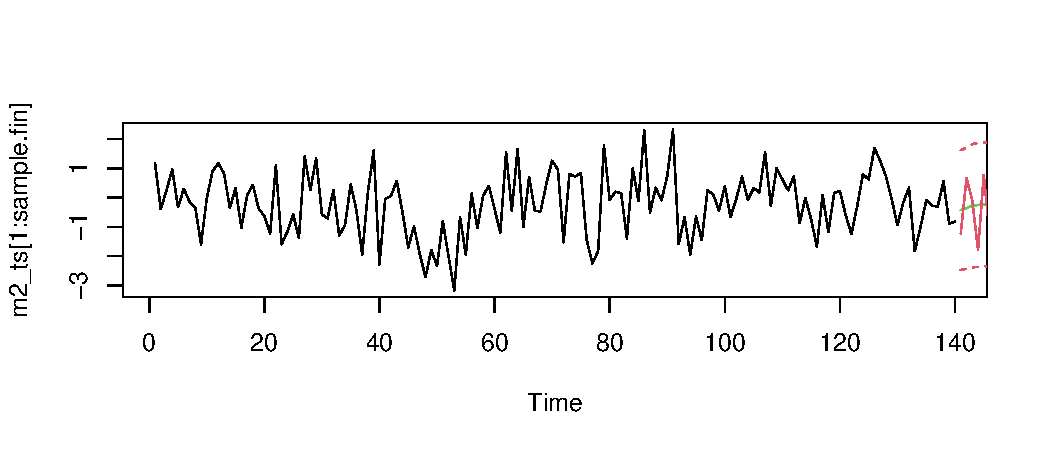
\includegraphics[width=0.9\linewidth]{RmdFigs/forecast1_m2-1} \end{center}

\hypertarget{otro-muxe9todo-para-pronuxf3stico-con-arma20}{%
\subsection{Otro método para pronóstico con
ARMA(2,0)}\label{otro-muxe9todo-para-pronuxf3stico-con-arma20}}

\begin{Shaded}
\begin{Highlighting}[]
\KeywordTok{library}\NormalTok{(forecast)}
\NormalTok{arima7<-}\StringTok{ }\KeywordTok{arima}\NormalTok{(m2_ts[}\DecValTok{1}\OperatorTok{:}\NormalTok{sample.fin], }\DataTypeTok{order =} \KeywordTok{c}\NormalTok{(}\DecValTok{2}\NormalTok{,}\DecValTok{0}\NormalTok{,}\DecValTok{0}\NormalTok{))}
\end{Highlighting}
\end{Shaded}

\begin{Shaded}
\begin{Highlighting}[]
\NormalTok{forecast7<-}\KeywordTok{forecast}\NormalTok{(arima7, }\DataTypeTok{level =} \KeywordTok{c}\NormalTok{(}\DecValTok{95}\NormalTok{), }\DataTypeTok{h =} \DecValTok{10}\NormalTok{)}
\KeywordTok{autoplot}\NormalTok{(forecast7)}
\end{Highlighting}
\end{Shaded}

\begin{center}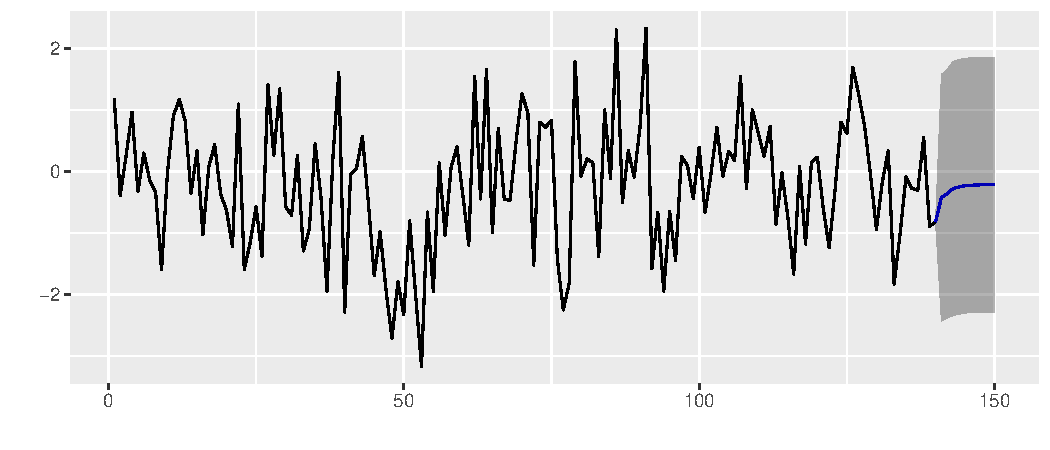
\includegraphics[width=0.9\linewidth]{RmdFigs/f_otro1-1} \end{center}

\hypertarget{comprobar-los-errores-de-los-pronuxf3sticos-con-arma20}{%
\subsection{Comprobar los errores de los pronósticos con
ARMA(2,0)}\label{comprobar-los-errores-de-los-pronuxf3sticos-con-arma20}}

\begin{Shaded}
\begin{Highlighting}[]
\KeywordTok{error}\NormalTok{(}\DataTypeTok{forecast=}\NormalTok{AR2_}\DecValTok{20}\NormalTok{_forecast, }\DataTypeTok{true=}\NormalTok{m2_ts[}\DecValTok{141}\OperatorTok{:}\DecValTok{150}\NormalTok{], }\DataTypeTok{method=}\KeywordTok{c}\NormalTok{(}\StringTok{"mse"}\NormalTok{))}
\end{Highlighting}
\end{Shaded}

\begin{verbatim}
## [1] 0.793164
\end{verbatim}

\begin{Shaded}
\begin{Highlighting}[]
\KeywordTok{error}\NormalTok{(}\DataTypeTok{forecast=}\NormalTok{AR2_}\DecValTok{20}\NormalTok{_forecast, }\DataTypeTok{true=}\NormalTok{m2_ts[}\DecValTok{141}\OperatorTok{:}\DecValTok{150}\NormalTok{], }\DataTypeTok{method=}\KeywordTok{c}\NormalTok{(}\StringTok{"mae"}\NormalTok{))}
\end{Highlighting}
\end{Shaded}

\begin{verbatim}
## [1] 0.766441
\end{verbatim}

\begin{Shaded}
\begin{Highlighting}[]
\KeywordTok{error}\NormalTok{(}\DataTypeTok{forecast=}\NormalTok{AR2_}\DecValTok{20}\NormalTok{_forecast, }\DataTypeTok{true=}\NormalTok{m2_ts[}\DecValTok{141}\OperatorTok{:}\DecValTok{150}\NormalTok{], }\DataTypeTok{method=}\KeywordTok{c}\NormalTok{(}\StringTok{"mape"}\NormalTok{))}
\end{Highlighting}
\end{Shaded}

\begin{verbatim}
## [1] 151.0832
\end{verbatim}

\clearpage

\hypertarget{prueba-del-segundo-mejor-modelo-arma11}{%
\subsection{Prueba del segundo mejor modelo
ARMA(1,1)}\label{prueba-del-segundo-mejor-modelo-arma11}}

Para validar el modelo se grafica el correlograma de los residuos para
comprobar que son ruido blanco.

\begin{Shaded}
\begin{Highlighting}[]
\CommentTok{# Calculo ACF y PACF para el mejor modelo ARMA para el dataset modelo2}
\NormalTok{res_m2_arma5 <-}\StringTok{ }\NormalTok{residuos.modelos[,}\DecValTok{5}\NormalTok{]}
\KeywordTok{acf2}\NormalTok{(res_m2_arma5)}
\end{Highlighting}
\end{Shaded}

\begin{center}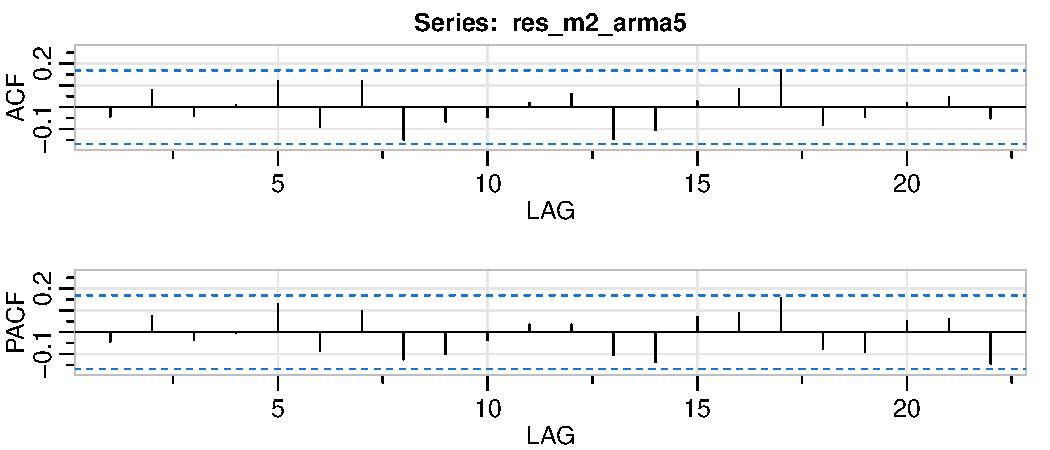
\includegraphics[width=0.9\linewidth]{RmdFigs/acf2_arma5-1} \end{center}

\begin{verbatim}
##       [,1] [,2]  [,3] [,4] [,5]  [,6] [,7]  [,8]  [,9] [,10] [,11] [,12] [,13]
## ACF  -0.04 0.08 -0.04 0.01 0.12 -0.09 0.12 -0.15 -0.07 -0.04  0.02  0.06 -0.15
## PACF -0.04 0.08 -0.04 0.00 0.13 -0.09 0.10 -0.12 -0.10 -0.03  0.03  0.03 -0.10
##      [,14] [,15] [,16] [,17] [,18] [,19] [,20] [,21] [,22]
## ACF  -0.10  0.03  0.08  0.17 -0.08 -0.04  0.02  0.05 -0.05
## PACF -0.14  0.07  0.09  0.16 -0.08 -0.09  0.05  0.06 -0.14
\end{verbatim}

En los correlogramas se aprecia que no hay ningún rezago significativo
por lo que se puede decir que los residuos son ruido blanco.

Por lo tanto estamos en condiciones de realizar un pronóstico para las
siguientes 10 observaciones de la serie.

\hypertarget{pronuxf3stico-para-modelo-2-con-arma11}{%
\subsection{Pronóstico para Modelo 2 con
ARMA(1,1)}\label{pronuxf3stico-para-modelo-2-con-arma11}}

\begin{Shaded}
\begin{Highlighting}[]
\CommentTok{#parametros p y q del mejor modelo}
\NormalTok{p <-}\StringTok{ }\DecValTok{1}
\NormalTok{q <-}\StringTok{ }\DecValTok{1}
\CommentTok{#fiteo el modelo con 140 datos (para despues hacer el out-of-sample forecast)}
\NormalTok{sample.fin <-}\StringTok{ }\DecValTok{140}
\NormalTok{AR2_}\DecValTok{11}\NormalTok{ <-}\StringTok{ }\KeywordTok{arima}\NormalTok{(m2_ts[}\DecValTok{1}\OperatorTok{:}\NormalTok{sample.fin], }\DataTypeTok{order =} \KeywordTok{c}\NormalTok{(p,}\DecValTok{0}\NormalTok{,q))}
\KeywordTok{ts.plot}\NormalTok{(m2_ts[}\DecValTok{1}\OperatorTok{:}\DecValTok{150}\NormalTok{])}
\end{Highlighting}
\end{Shaded}

\begin{center}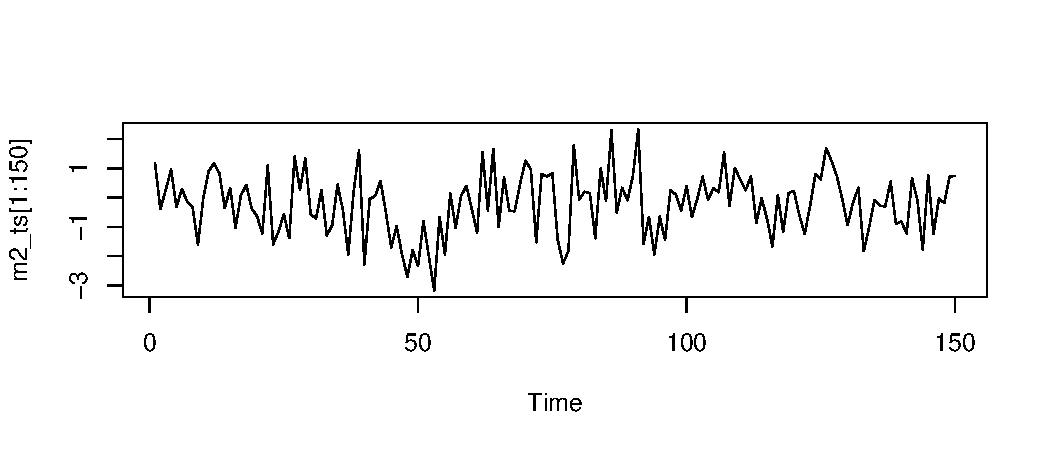
\includegraphics[width=0.9\linewidth]{RmdFigs/fit_2_m2-1} \end{center}

\begin{Shaded}
\begin{Highlighting}[]
\CommentTok{#plotting the m2_ts series plus the forecast and 95% prediction intervals}
\KeywordTok{ts.plot}\NormalTok{(m2_ts[}\DecValTok{1}\OperatorTok{:}\NormalTok{sample.fin], }\DataTypeTok{xlim =} \KeywordTok{c}\NormalTok{(}\DecValTok{1}\NormalTok{, sample.fin))}
\NormalTok{AR2_}\DecValTok{11}\NormalTok{_forecast <-}\StringTok{ }\KeywordTok{predict}\NormalTok{(AR2_}\DecValTok{11}\NormalTok{, }\DataTypeTok{n.ahead =} \KeywordTok{length}\NormalTok{(m2_ts)}\OperatorTok{-}\NormalTok{sample.fin)}\OperatorTok{$}\NormalTok{pred}
\NormalTok{AR2_}\DecValTok{11}\NormalTok{_forecast_se <-}\StringTok{ }\KeywordTok{predict}\NormalTok{(AR2_}\DecValTok{11}\NormalTok{, }\DataTypeTok{n.ahead =} \KeywordTok{length}\NormalTok{(m2_ts)}\OperatorTok{-}\NormalTok{sample.fin)}\OperatorTok{$}\NormalTok{se}
\KeywordTok{points}\NormalTok{(AR2_}\DecValTok{11}\NormalTok{_forecast, }\DataTypeTok{type =} \StringTok{"l"}\NormalTok{, }\DataTypeTok{col =} \DecValTok{2}\NormalTok{)}
\KeywordTok{points}\NormalTok{(AR2_}\DecValTok{11}\NormalTok{_forecast }\OperatorTok{-}\StringTok{ }\DecValTok{2}\OperatorTok{*}\NormalTok{AR2_}\DecValTok{11}\NormalTok{_forecast_se, }\DataTypeTok{type =} \StringTok{"l"}\NormalTok{, }\DataTypeTok{col =} \DecValTok{2}\NormalTok{, }\DataTypeTok{lty =} \DecValTok{2}\NormalTok{)}
\KeywordTok{points}\NormalTok{(AR2_}\DecValTok{11}\NormalTok{_forecast }\OperatorTok{+}\StringTok{ }\DecValTok{2}\OperatorTok{*}\NormalTok{AR2_}\DecValTok{11}\NormalTok{_forecast_se, }\DataTypeTok{type =} \StringTok{"l"}\NormalTok{, }\DataTypeTok{col =} \DecValTok{2}\NormalTok{, }\DataTypeTok{lty =} \DecValTok{2}\NormalTok{)}
\KeywordTok{points}\NormalTok{(sample.fin}\OperatorTok{+}\DecValTok{1}\OperatorTok{:}\DecValTok{150}\NormalTok{,m2_ts[sample.fin}\OperatorTok{+}\DecValTok{1}\OperatorTok{:}\DecValTok{150}\NormalTok{], }\DataTypeTok{type =} \StringTok{"l"}\NormalTok{, }\DataTypeTok{col =} \DecValTok{3}\NormalTok{)}
\end{Highlighting}
\end{Shaded}

\begin{center}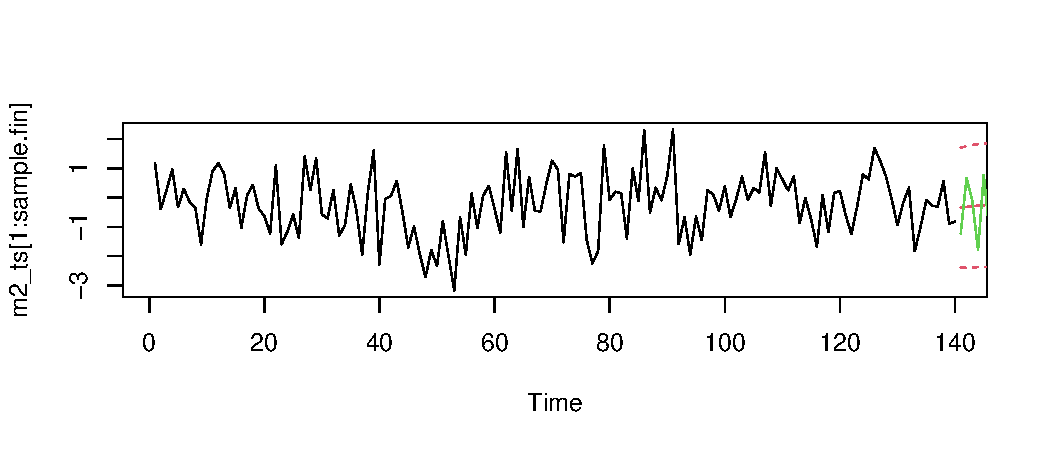
\includegraphics[width=0.9\linewidth]{RmdFigs/forecast2_m5-1} \end{center}

\hypertarget{otro-muxe9todo-para-pronuxf3stico-con-arma11}{%
\subsection{Otro método para pronóstico con
ARMA(1,1)}\label{otro-muxe9todo-para-pronuxf3stico-con-arma11}}

\begin{Shaded}
\begin{Highlighting}[]
\KeywordTok{library}\NormalTok{(forecast)}
\NormalTok{arima5<-}\StringTok{ }\KeywordTok{arima}\NormalTok{(m2_ts[}\DecValTok{1}\OperatorTok{:}\NormalTok{sample.fin], }\DataTypeTok{order =} \KeywordTok{c}\NormalTok{(}\DecValTok{1}\NormalTok{,}\DecValTok{0}\NormalTok{,}\DecValTok{1}\NormalTok{))}
\end{Highlighting}
\end{Shaded}

\begin{Shaded}
\begin{Highlighting}[]
\NormalTok{forecast5<-}\KeywordTok{forecast}\NormalTok{(arima5, }\DataTypeTok{level =} \KeywordTok{c}\NormalTok{(}\DecValTok{95}\NormalTok{), }\DataTypeTok{h =} \DecValTok{10}\NormalTok{)}
\KeywordTok{autoplot}\NormalTok{(forecast5)}
\end{Highlighting}
\end{Shaded}

\begin{center}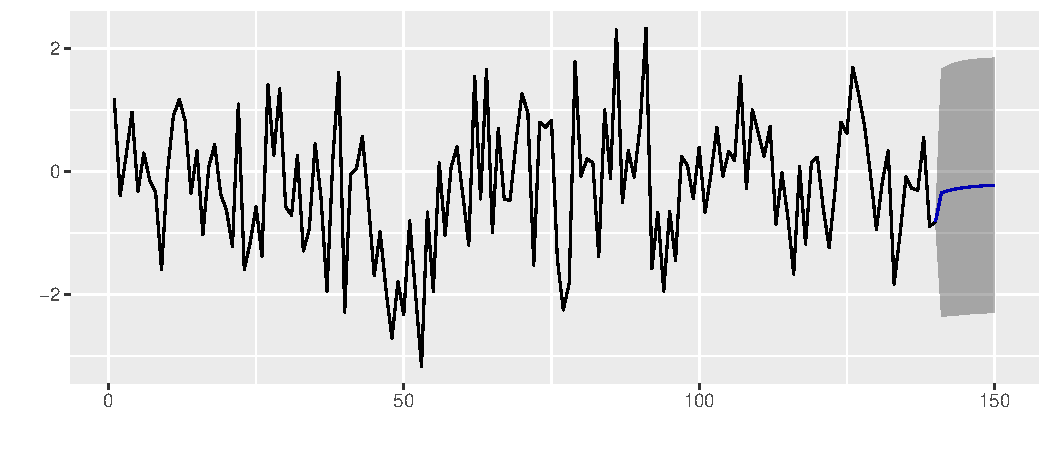
\includegraphics[width=0.9\linewidth]{RmdFigs/f_otro2_2-1} \end{center}

\hypertarget{comprobar-los-errores-de-los-pronuxf3sticos-con-arma11}{%
\subsection{Comprobar los errores de los pronósticos con
ARMA(1,1)}\label{comprobar-los-errores-de-los-pronuxf3sticos-con-arma11}}

\begin{Shaded}
\begin{Highlighting}[]
\KeywordTok{error}\NormalTok{(}\DataTypeTok{forecast=}\NormalTok{AR2_}\DecValTok{11}\NormalTok{_forecast, }\DataTypeTok{true=}\NormalTok{m2_ts[}\DecValTok{141}\OperatorTok{:}\DecValTok{150}\NormalTok{], }\DataTypeTok{method=}\KeywordTok{c}\NormalTok{(}\StringTok{"mse"}\NormalTok{))}
\end{Highlighting}
\end{Shaded}

\begin{verbatim}
## [1] 0.797546
\end{verbatim}

\begin{Shaded}
\begin{Highlighting}[]
\KeywordTok{error}\NormalTok{(}\DataTypeTok{forecast=}\NormalTok{AR2_}\DecValTok{11}\NormalTok{_forecast, }\DataTypeTok{true=}\NormalTok{m2_ts[}\DecValTok{141}\OperatorTok{:}\DecValTok{150}\NormalTok{], }\DataTypeTok{method=}\KeywordTok{c}\NormalTok{(}\StringTok{"mae"}\NormalTok{))}
\end{Highlighting}
\end{Shaded}

\begin{verbatim}
## [1] 0.776066
\end{verbatim}

\begin{Shaded}
\begin{Highlighting}[]
\KeywordTok{error}\NormalTok{(}\DataTypeTok{forecast=}\NormalTok{AR2_}\DecValTok{11}\NormalTok{_forecast, }\DataTypeTok{true=}\NormalTok{m2_ts[}\DecValTok{141}\OperatorTok{:}\DecValTok{150}\NormalTok{], }\DataTypeTok{method=}\KeywordTok{c}\NormalTok{(}\StringTok{"mape"}\NormalTok{))}
\end{Highlighting}
\end{Shaded}

\begin{verbatim}
## [1] 160.3067
\end{verbatim}

\end{document}
